\documentclass{article}
% bibliography setup
\usepackage{natbib}
\bibliographystyle{apalike}  % abbrvnat
\setcitestyle{authoryear,open={(},close={)}} %Citation-related commands
% makes color citations
\usepackage[colorlinks=true,urlcolor=blue,citecolor=red,linkcolor=red,bookmarks=true]{hyperref}
% images
\usepackage{graphicx}
\graphicspath{ {./images/} }

% hypter parameter setup
\usepackage{hyperref}
% for table setup
\usepackage{tabularx}

\title{Improved Sequential Hypothesis Testing with
``Enhanced Precision Is The Goal"}
\date{\today}
\author{Eyal A. Kazin}

\begin{document}
\maketitle

\input precision_goal_abstract

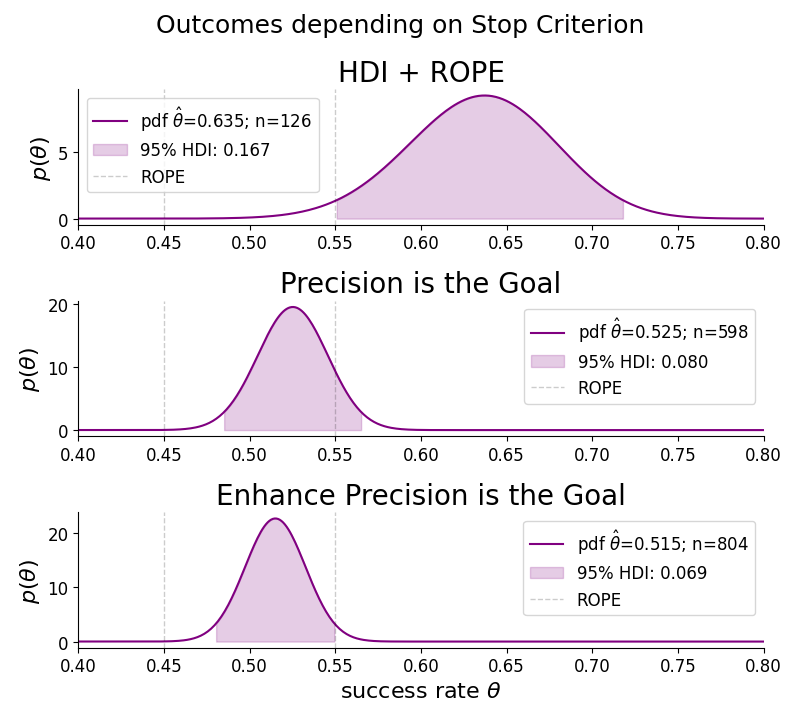
\includegraphics[scale=0.5]{cherry_posteriors.png}

%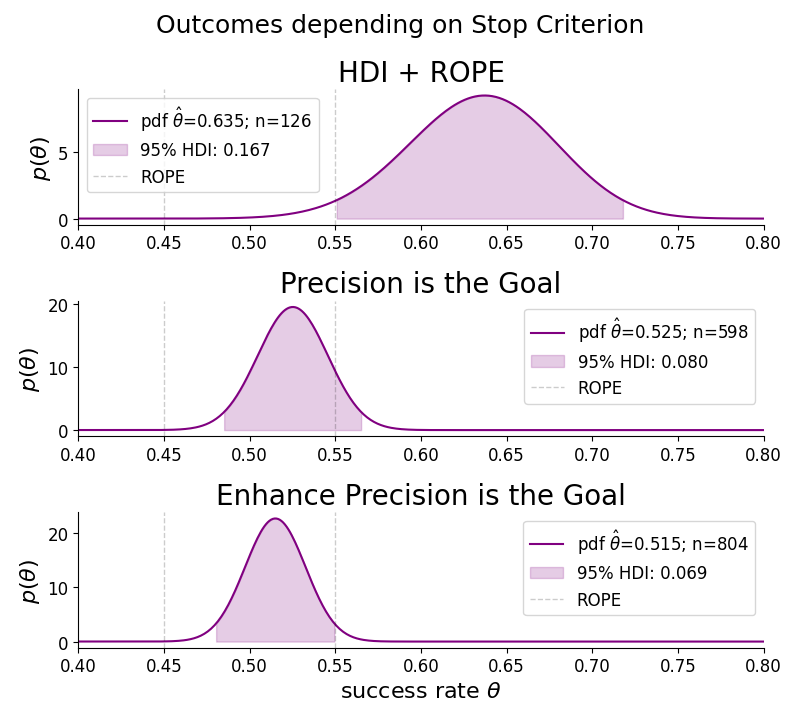
\includegraphics[width=1\textwidth]{cherry_posteriors.png}

\begin{figure}[h]
    \centering
    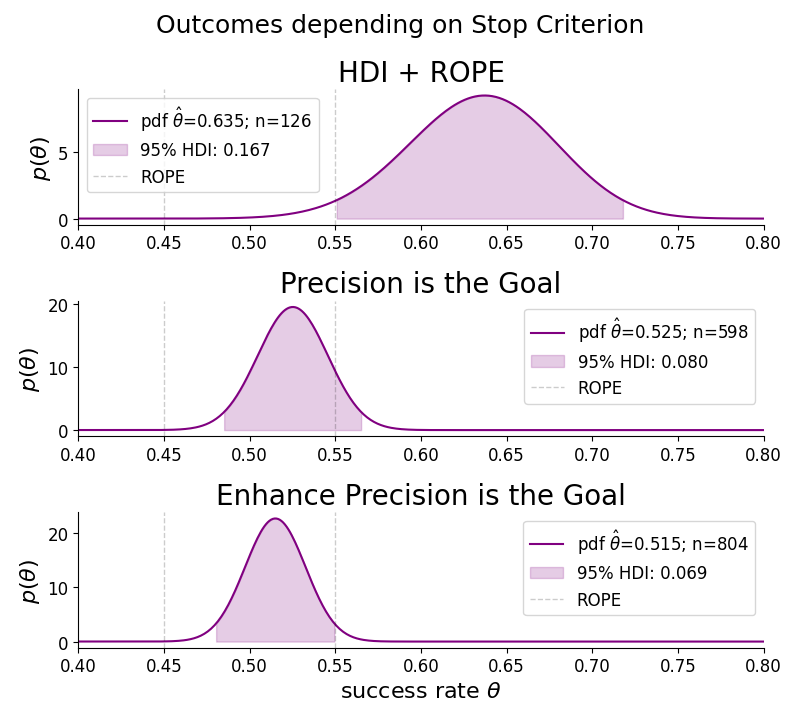
\includegraphics[width=1\textwidth]{cherry_posteriors.png}
    \caption{Beta function posteriors of subsamples of example sequence from Figure REF. Panels are results of different stop/decision criteria being triggered. Shaded areas are 95\% HDIs. ROPE within vertical dashed lines.
    Top - HDI+ ROPE triggers when the 95\% HDI is fully outside the ROPE (iteration 126). Incorrectly rejects $\theta_{\rm null}$. Middle - “Precision is the Goal” triggers when 95\% HDI width reaches precision goal of 80\% ROPE width (iteration 598). HDI straddles the ROPE → inconclusive.
    Bottom - “Enhanced Precision is the Goal” triggers when 95\% HDI fully within ROPE and obtains same precision goal (iteration 804). Correctly accepts $\theta_{\rm null}$}
\end{figure}

\section{Introduction}
\input precision_goal_introduction

\subsection{Contributions}

\subsubsection{Paper Structure}
The paper is organized as follows.
In the Methods section we describe three (four if Frequentist?)
stop criteria as well as the setup to test on synthetic deichotomous data.
In the Results section we present the results of the synthetic data analysis as well as analytical analysis.
In the Discussion section we discuss the implications of the results (Reword this).
In the Conclusion section we summarize the findings and suggest future directions (Reword this).


\section{Methods}

Here we describe three stopping algorithms for sequential hypothesis testing.

We begine by describing heuristics of posterior location and width used in all three.
We describe their intuition, as well as in pseudo code.
We also provide useful anlaytical experessions and conclude by describing a setup
to test the methods on synthetic data.
Although our belief is that these methods apply to any type of data,
our focus is on dichotomous data (Bernouli trials)
in order to compare with \cite{kruschke2015doing}
(somehow experess that: "as it is simple to describe analytically and
to conduct rapid tests on synthetic data.")

We conclude with a contrast comparison of the algorithms.

(Mention somewhere difference between "stopping algorithm" to "stopping criterion",
perhaps "collection algorithm"?)


\subsubsection{Region of Practical Equivalence and High Density Interval}
All three stop algorithms explored below depend on heuristics that describe two key
aspects of expectations from the experiment:
\begin{itemize}
    \item Effective size expected from the experiment
    \item Posterior width
\end{itemize}


One common misconception in hypothesis testing is that an outcome that is
“statistically significant” is sufficient to make a meaningful real world decision.
In practice one must consider the effect size.
E.g, medical research requires a “minimal detectable change” or
“minimal clinically important difference” to consider an outcome relevant for
considering a change in action.

As an over simplistic made-up example imagine that a researcher examines if a
therapeutic differs in impact by gender.
If we assume that enough data was collected to demonstrate that the difference is
“statistically significant”, e.g, that the drug is 72.1\% beneficial for males
and 72.3\% for females, a practitioner, depending on circumstance may consider
this equivalent for all practical purposes.
To justify treating the usage of the drug by gender the
researcher (or the board of the company or a regulatory body) would demand
a meaningful absolute difference e.g,  5\% or 10\% or more
(depending on the context, e.g, for purposes of further research, or approval
of the drug). Hence the researcher should define in advance of collecting data an
“effective area" around the null hypothesis being examined to determine if a
decision making difference is present.

One such metric of interest to account for the importance of the effective size
is referred to as the
\textit{Region of Practical Equivalence} (ROPE).
The ROPE is defined as an area around the null value considered “similar enough 
to the null hypothesis" such that if the true value is within this area by all
means it is effectively the same to the null hypothesis.

The width of the ROPE depends on the task at hand.
E.g, consider the precision of the fairness of dice required in a family board game
against that required for gambling enterprises.
A manufacturer of household board games would like them to be fair to a certain extent,
but would not want to pay a premium for accuracy that would not be noticed by a casual
player. A casino on the other hand would require a much higher accuracy to ensure
players that the dice are not loaded.

In the algorithms expolred here we are intersted in the quantifying the overlap
between the posterior and the ROPE, e.g a \textit{credible interval} (similar to the frequentist confidence interval).
A popular heuristic is the \textit{Highest Density Interval} (HDI)
which describes the region where a substantial amount of the posterior resides.
In practice the HDI means that all points within the credible interval have a higher
probability density than points outside of it.

The width of the HDI is commonly calculated using 95\% of the mass to be comparable
with that used traditionally in Frequentist hypothesis testing.
Whereas this is reasonable for analytical solutions (i.e, solved using an equation),
for numerical solutions it has been shown that for high precision 10,000 samples are
required, otherwise one should use a lower mass percentage like 94\% (Kruschke, 2014, look up BIB).
\cite{mcelreath2016} suggests 89\% as a quip to the arbitrariness of the importance of the
width of the credible interval, where the only noteworthy feature of this value is being
the highest prime value under the traditional 95\% threshold.  

The ROPE and HDI metrics may be used in various combinations in the stop algorithm.
The common factor in all three that we discuss here is their decision criterion
which we discuss next.


\subsubsection{Decision Criterion: Is The HDI In Or Out Of The ROPE?}

\subsubsection{HDI + ROPE: Location, Location, Location}

\subsubsection{Algorithm Intuition And Comparison}

all of which rely on the same decision criterion to determine acceptence
or rejection of the null hypothesis.




Table (cite table) provides an intuitive comparison between the three algorithms of interst.
In order to conduct this comparison we consider:
\begin{itemize}
    \item Pre Survey Decisions - the parameters required to decide ahead of data
    collection
    \item The stop criterion main characteristic 
    \item The decision criterion characteristic
    \item Stop and Decision order - are they simultaneous a two step process?
\end{itemize}
By creterion {\it characteristic} we are referring to the property of the posterior of
importance: its location and/or width

% make a table in latex with four rows and 5 columns

\begin{tabularx}{1.2\textwidth} { 
    | >{\raggedright\arraybackslash}X 
    | >{\centering\arraybackslash}X 
    | >{\raggedright\arraybackslash}X 
    | >{\centering\arraybackslash}X 
    | >{\raggedleft\arraybackslash}X | }
   \hline
   Algorithm & Pre Survey Decisions & Stop Criterion Characteristic

   & Decision Criterion Characteristic & Sequence\\
   \hline
   HDI + ROPE  & \textbf{$N_\mathrm{min}$}, $N_\mathrm{max}$, $\sigma_\mathrm{effect}$  & Location  & Location & Simultaneously \\
   \hline
   item 31  & item 32  & item 33  & item 34 \\
   
  \hline
  \end{tabularx}
\\
\\
\\
Here we use notation

  \begin{itemize}
        \item $N_\mathrm{min}$ - the minimal sample size to collect (needs further explanation)
        \item $N_\mathrm{max}$ - the maximum sample size
        \item $\sigma_\mathrm{effect}$ - The effect size
         
  \end{itemize}



\subsubsection{Enhanced Precision Is The Goal: Width \& Location}

\subsection{Synthetic Data Analysis}


\section{Results}

\section{Discussion}

\section{Conclusion}

\section{Useful Equations}
\input precision_goal_useful_equations

\section{Submission Instructions}

Methods Paper—maximum word count: 6500
Methods Papers present an advance likely to make major impact in one or more applied
fields. While theory (e.g. theorems concerning statistical or
learning-theoretic properties) are welcome, this is not essential, but intuition and
understanding of why the method works is important.
We are also very open to theory in a broader sense including examples and conjectures.
Generally, we would expect empirical results to demonstrate effectiveness.
However, in cases where the extent of methodological/conceptual innovation is large
enough, results themselves may be illustrative and need not be of immediate high impact
in any particular applied domain.

Each piece should include:

Unstructured Abstract—maximum word count: 250
Keywords—maximum of 6 and minimum of 5
May include tables and figures—no limit
May include the following back matter sections:
Acknowledgements
Author contributions (with CRediT details)
Conflicts of interest
Funding
Must include the following:
Data availability
References—no limit
Each submission must contain the following sections and use these terms as the first
level section headers: Introduction, Methods, Results, Discussion and Conclusion
(Discussion and Conclusion may be combined).

{\bf Resources}

\href{https://academic.oup.com/rssdat/pages/general-instructions}{RSS Instructions} 

\href{https://academic.oup.com/pages/authoring/books/preparing-your-manuscript/working-in-latex}{RSS Working in \LaTeX}.

\bibliography{references.bib}

\end{document}